\chapter{From raw specification to fully proven spec: A full example}
\label{ch:fullexample}

In this chapter we take a system specification through all the steps of \gls{zmath} to demonstrate how we can get from a raw specification to a full proof. We have added commentary throughout so the reader can understand how we can get from one step to another. We have added figures and screenshots of each step of the \gls{zmath} framework.

\section{Raw Specification}
We take a raw specification of a vending machine (shown in figure \ref{fig:rawschema}) The output for the specification can be seen in figure \ref{fig:rawschemaout}. The full input for this can be found in appendx \ref{app:vmspec}.

\begin{figure}[H]
\vspace{-0.2in}
\centering
\begin{minipage}{0.45\textwidth}
\centering
\begin{tiny}
\begin{BVerbatim}
\begin{zed}
price:\nat
\end{zed}
\begin{schema}{VMSTATE}
stock, takings: \nat
\end{schema}
\begin{schema}{VM\_operation}
\Delta VMSTATE \\
cash\_tendered?, cash\_refunded!: \nat \\
bars\_delivered! : \nat
\end{schema}
\begin{schema}{exact\_cash}
cash\_tendered?: \nat
\where
cash\_tendered? = price
\end{schema}
\begin{schema}{some\_stock}
stock: \nat
\where
stock > 0
\end{schema}
\begin{schema}{VM\_sale}
VM\_operation
\where
stock' = stock -1 \\
bars\_delivered! = 1 \\
cash\_refunded! = cash\_tendered? - price \\
takings' = takings + price
\end{schema}
\begin{zed}
VM1 \defs exact\_cash \land 
some\_stock \land VM\_sale
\end{zed}
\end{BVerbatim}
\end{tiny}
\vspace{-0.18in}
\caption{Part of the raw schema.\label{fig:rawschema}}
\vspace{-0.2in}
\end{minipage}\hfill
\begin{minipage}{0.45\textwidth}
\centering
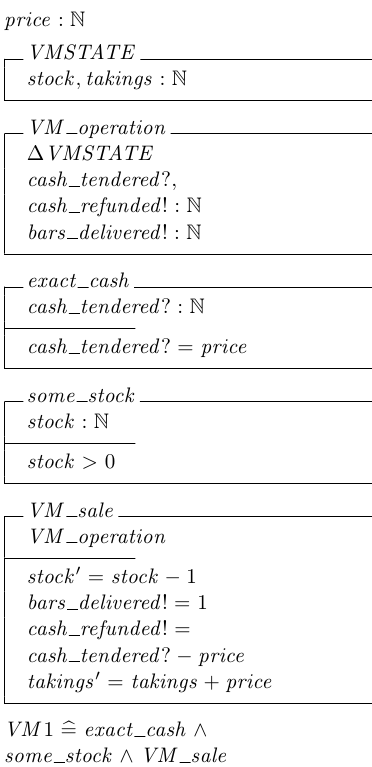
\includegraphics[scale=0.4]{Figures/fullexample/raw.png}
\vspace{-0.2in}
\caption{Part of a raw specification output. \label{fig:rawschemaout}}
\vspace{-0.2in}
\end{minipage}
\end{figure}


\section{ZCGa}

The user then goes to label the raw specification with the \gls{zcga} labels. The labelled specification can be seen in figure \ref{fig:zcgaschema}. The words highlighted in red are the \gls{zcga} annotations done by the user and the black text is the existing specification. Figure \ref{fig:zcgaschema} outputting result can be seen in figure \ref{fig:zcgaschemaout}.

\begin{figure}[H]
\centering
\begin{minipage}{0.45\textwidth}
\centering
\begin{tiny}
\begin{BVerbatim}[commandchars=+\[\]]
\begin{zed}
[+color[red]\text{\declaration{
\term{]price[+color[red]}]:[+color[red]\expression{]\nat[+color[red]}}}]
\end{zed}
\begin{schema}{VMSTATE}
[+color[red]\text{\declaration{
\term{]stock[+color[red]}], [+color[red]\term{]takings[+color[red]}]:
[+color[red]\expression{]\nat[+color[red]}}}]
\end{schema}
\begin{schema}{VM\_operation}
[+color[red]\text{]\Delta VMSTATE[+color[red]}] \\
[+color[red]\text{\declaration{
\term{]cash\_tendered?[+color[red]}]:[+color[red]\expression{]\nat[+color[red]}}}] \\
[+color[red]\text{\declaration{
\term{]cash\_refunded![+color[red]}]:[+color[red]\expression{]\nat[+color[red]}}}] \\
[+color[red]\text{\declaration{
\term{]bars\_delivered![+color[red]}]:[+color[red]\expression{]\nat[+color[red]}}}]
\end{schema}
\begin{schema}{exact\_cash}
[+color[red]\text{\declaration{
\term{]cash\_tendered?[+color[red]}]:[+color[red]\expression{]\nat[+color[red]}}}]
\where
[+color[red]\text{\expression{
\term{]cash\_tendered?[+color[red]}] = [+color[red]\term{]price[+color[red]}}}]
\end{schema}
\begin{schema}{some\_stock}
[+color[red]\text{\declaration{
\term{]stock[+color[red]}]:[+color[red]\expression{]\nat[+color[red]}}}]
\where
[+color[red]\text{\expression{
\term{]stock[+color[red]}] > [+color[red]\term{]0[+color[red]}}}]
\end{schema}
\begin{schema}{VM\_sale}
[+color[red]\text{]VM\_operation[+color[red]}]
\where
[+color[red]\text{\expression{
\term{]stock'[+color[red]}] = [+color[red]\term{\term{]stock[+color[red]}]-[+color[red]\term{]1[+color[red]}}}}] \\
[+color[red]\text{\expression{
\term{]bars\_delivered![+color[red]}]=[+color[red]\term{]1[+color[red]}}}] \\
[+color[red]\text{\expression{
\term{]cash\_refunded![+color[red]}]= 
[+color[red]\term{]cash\_tendered?[+color[red]}]-[+color[red]\term{]price[+color[red]}}}] \\
[+color[red]\text{\expression{
\term{]takings'[+color[red]}]=[+color[red]\term{]takings[+color[red]}]\plus [+color[red]\term{]price[+color[red]}}}]
\end{schema}
\begin{zed}
VM1 \defs [+color[red]\text{\expression{\text{]exact\_cash[+color[red]}] \land 
[+color[red]\text{]some\_stock[+color[red]}] \land [+color[red]\text{]VM\_sale[+color[red]}}}]
\end{zed}
\end{BVerbatim}
\end{tiny}
\vspace{-0.2in}
\caption{Part of the raw schema.\label{fig:zcgaschema}}
\vspace{-0.2in}
\end{minipage}\hfill
\begin{minipage}{0.45\textwidth}
\centering
\centering
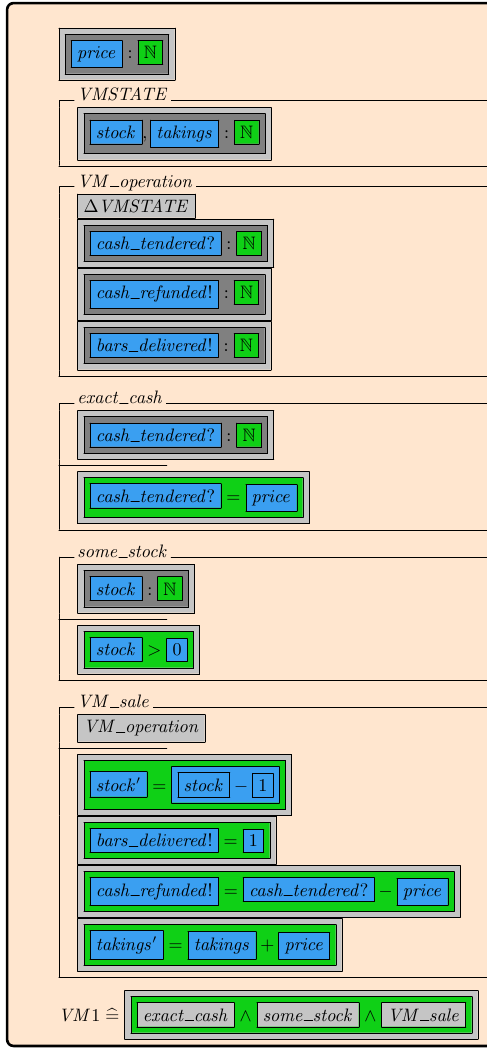
\includegraphics[scale=0.4]{Figures/fullexample/zcga.png}
\vspace{-0.2in}
\caption{Part of a ZCGa labelled specification output. \label{fig:zcgaschemaout}}
\end{minipage}
\end{figure}

After annotating we run it through the \gls{zcga} correctness checker. Figure \ref{fig:zcgacorrect} shows the message which appears when the annotated specification has been checked. 

\begin{figure}[H]
\centering
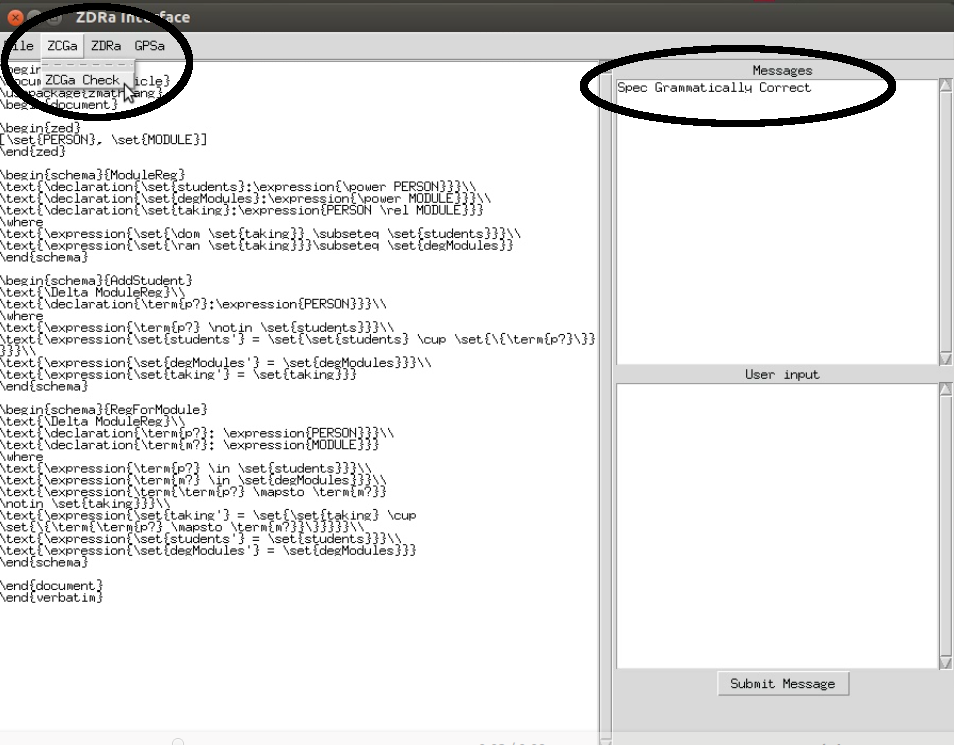
\includegraphics[scale=0.3]{Figures/fullexample/zcgacorrect.png}
\caption{Message which appears after running the ZCGa checker on our example. \label{fig:zcgacorrect}}
\end{figure}

\section{ZDRa}

Next the user can add \gls{zdra} relations to chuk parts of the specification together and add relations to them. Figure \ref{fig:zdrazcgaAno} shows our example labelled in \gls{zdra} annotations (in blue), the \gls{zcga} annotations are in grey and existing specification in black. Figure \ref{fig:zdrazcgaout} shows the compiled result.

\begin{figure}[H]
\vspace{-0.2in}
\centering
\begin{minipage}{0.45\textwidth}
\centering
\begin{tiny}
\begin{BVerbatim}[commandchars=+\[\]]
[+color[blue]\dratheory{T1}{0.5}{]
\begin{zed}
[+color[gray]\text{\declaration{\term{]price[+color[gray]}]: [+color[gray]\expression{]\nat[+color[gray]}}}]
\end{zed}
[+color[blue]\draschema{SS1}{]
\begin{schema}{VMSTATE}
[+color[gray]\text{\declaration{\term{]stock[+color[gray]}],
[+color[gray]\term{]takings[+color[gray]}]: [+color[gray]\expression{]\nat[+color[gray]}}}]
\end{schema}[+color[blue]}]
[+color[blue]\draschema{CS0}{]
\begin{schema}{VM\_operation}
[+color[gray]\text{]\Delta VMSTATE[+color[gray]}] \\
[+color[gray]\text{\declaration{\term{]cash\_tendered?[+color[gray]}], 
[+color[gray]\term{]cash\_refunded![+color[gray]}]: [+color[gray]\expression{]\nat[+color[gray]}}}] \\
[+color[gray]\text{\declaration{\term{]bars\_delivered![+color[gray]}]:
[+color[gray]\expression{]\nat[+color[gray]}}}]
\end{schema}[+color[blue]}]
[+color[blue]\uses{CS0}{SS1}]
[+color[blue]\draschema{PRE1}{]
\begin{schema}{exact\_cash}
[+color[gray]\text{\declaration{\term{]cash\_tendered?[+color[gray]}]:
[+color[gray]\expression{]\nat[+color[gray]}}}]
\where
[+color[gray]\text{\expression{]
[+color[gray]\term{]cash\_tendered?[+color[gray]}] = [+color[gray]\term{]price[+color[gray]}}}]
\end{schema}[+color[blue]}]
[+color[blue]\draschema{PRE2}{]
\begin{schema}{some\_stock}
[+color[gray]\text{\declaration{\term{]stock[+color[gray]}]: [+color[gray]\expression{]\nat[+color[gray]}}}]
\where
[+color[gray]\text{\expression{\term{]stock[+color[gray]}] > [+color[gray]\term{]0[+color[gray]}}}]
\end{schema}[+color[blue]}]
[+color[blue]\draschema{CS1}{]
\begin{schema}{VM\_sale}
[+color[gray]\text{]VM\_operation[+color[gray]}]
\where
[+color[blue]\draline{PO1}{]
[+color[gray]\text{\expression{\term{]stock'[+color[gray]}] =
[+color[gray]\term{\term{]stock[+color[gray]}] - [+color[gray]\term{]1[+color[gray]}}}}] \\
[+color[gray]\text{\expression{\term{]bars\_delivered![+color[gray]}] = [+color[gray]\term{]1[+color[gray]}}}] \\
[+color[gray]\text{\expression{\term{]cash\_refunded![+color[gray]}] =
[+color[gray]\term{\term{]cash\_tendered?[+color[gray]}] - [+color[gray]\term{]price[+color[gray]}}}}] \\
[+color[gray]\text{\expression{\term{]takings'[+color[gray]}] =
[+color[gray]\term{]takings[+color[gray]}] \plus [+color[gray]\term{]price[+color[gray]}}]}[+color[blue]}]
\end{schema}[+color[blue]}]
[+color[blue]\requires{CS1}{PO1}
\uses{CS1}{CS0}
\draschema{TS1}{]
\begin{zed}
VM1 \defs [+color[gray]\text{\expression{\text{]exact\_cash[+color[gray]}] 
\land [+color[gray]\text{]some\_stock[+color[gray]}] \land [+color[gray]\text{]VM\_sale[+color[gray]}}}]
\end{zed}[+color[blue]}]
[+color[blue]\uses{TS1}{PRE1}
\uses{TS1}{PRE2}
\uses{TS1}{CS1}}]
\end{BVerbatim}
\end{tiny}
\vspace{-0.18in}
\caption{An example of a specification labelled in \gls{zcga} and \gls{zdra}.).\label{fig:zdrazcgaAno}}
\vspace{-0.2in}
\end{minipage}\hfill
\begin{minipage}{0.45\textwidth}
\centering
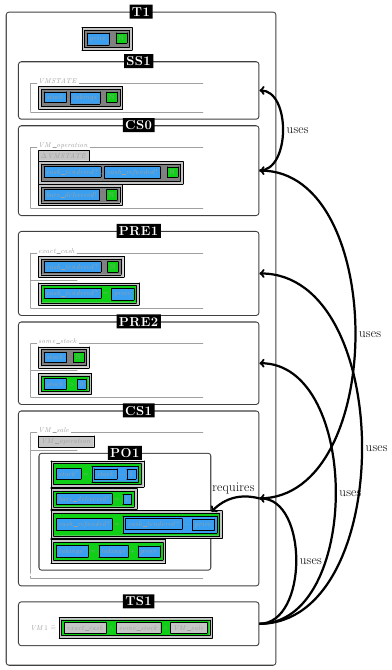
\includegraphics[scale=0.55]{Figures/fullexample/zdra.png}
\vspace{-0.18in}
\caption{An example of a specification output labelled in \gls{zcga} and \gls{zdra}.).\label{fig:zdrazcgaout}}
\vspace{-0.2in}
\end{minipage}
\end{figure}

After annotating our example in \gls{zdra} labels we can then run our specification through the \gls{zdra} checker. Figure \ref{fig:zdracorrect} shows the message which appears after we check our example with \gls{zdra}.

\begin{figure}[H]
\centering
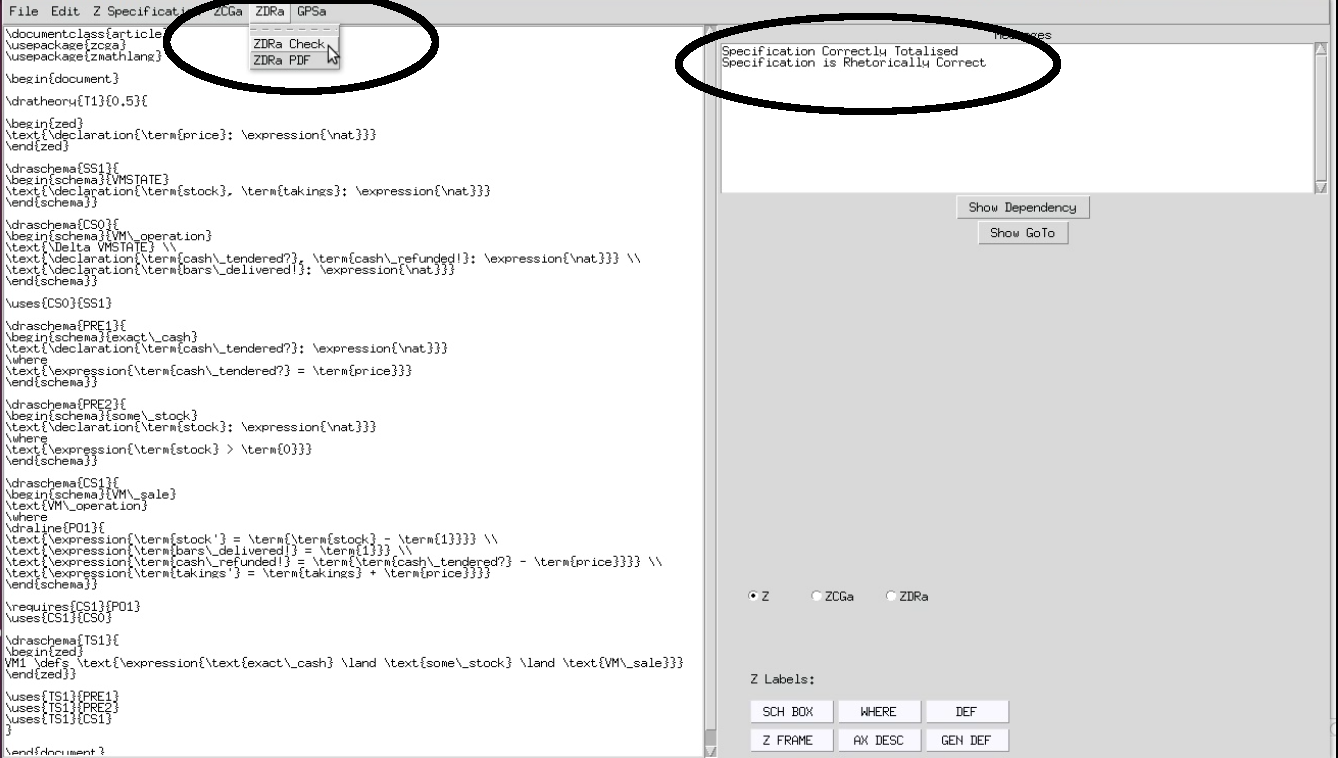
\includegraphics[scale=0.3]{Figures/fullexample/zdracorrect.png}
\caption{Message which appears after running the ZDRa checker on our example. \label{fig:zdracorrect}}
\end{figure}

\section{Graphs}

Since the example is \gls{zdra} correct the two graphs shown in figures \ref{fig:depexample} and \ref{fig:gotoexample} are automatically produced and saved on the users computer.

\begin{figure}[H]
\centering
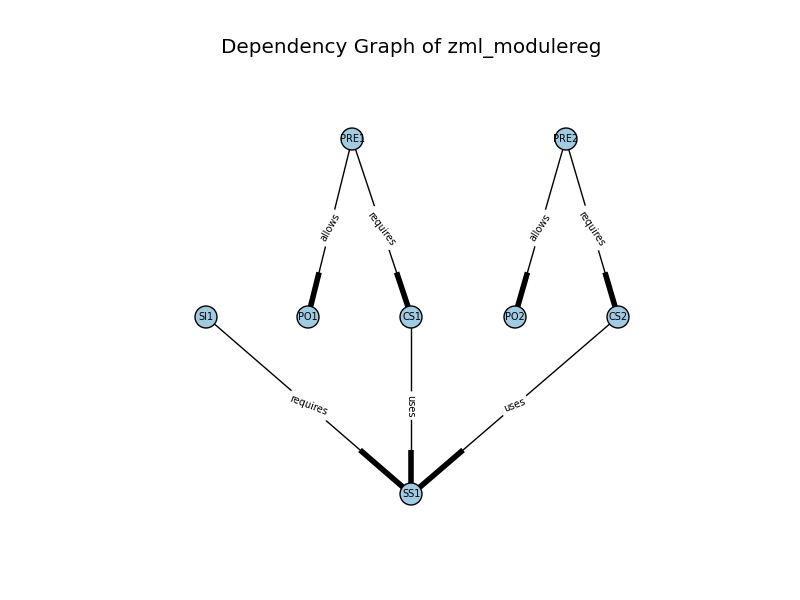
\includegraphics[scale=0.5]{Figures/fullexample/dp_fullexample.png}
\caption{Dependency graph automatically generated from the ZDRa for our example. \label{fig:depexample}}
\end{figure}

\begin{figure}[H]
\centering
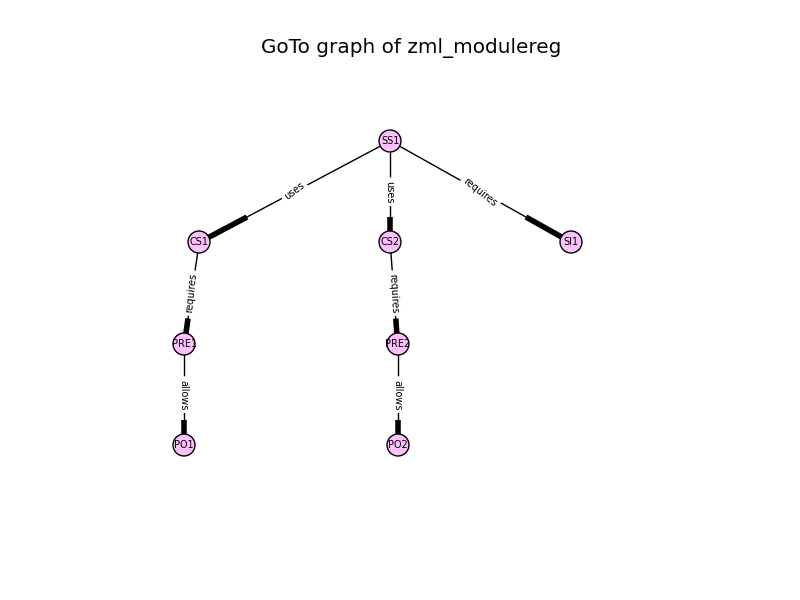
\includegraphics[scale=0.5]{Figures/fullexample/goto_fullexample.jpg}
\caption{GoTo graph automatically generated from the ZDRa for our example. \label{fig:gotoexample}}
\end{figure}

\section{Skeletons}

The skeletons are automatically generated if the specification passes the \gls{zcga} and \gls{zdra} check.

\subsection{General Proof Skeleton}

We can generate a general proof skeleton which prints out the \gls{zdra} name and the instances they should be converted to when inputting into any theorem prover. If the specification is \gls{zdra}] correct we can then generate the \gls{gpsa} by clicking on the \gls{gpsa} menu in the interface (figure \ref{fig:gpsabutton}).

\begin{figure}[H]
\centering
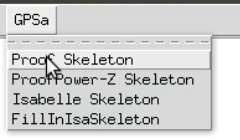
\includegraphics[scale=0.45]{Figures/fullexample/gpsa.png}
\caption{The GPSa button the interface which allows the user to generate the general proof skeleton. \label{fig:gpsabutton}}
\end{figure}

Figure \ref{fig:gpsaFullexample} shows the general proof skeleton which was generated for our example.

\begin{figure}[H]
\centering
\begin{scriptsize}
\begin{BVerbatim}
stateSchema SS1 
precondition PRE2 
precondition PRE1 
changeSchema CS0 
changeSchema CS1 
postcondition PO1 
lemma TS1 
\end{BVerbatim}
\end{scriptsize}
\caption{General proof skeleton. \label{fig:gpsaFullexample}}
\end{figure}

\subsection{Isabelle Skeleton}

From the general proof skeleton the ZMathLang program can automatically generate an Isabelle Skeleton. The user can do this by clicking on the \gls{gpsa} menu on the interface then clicking `\texttt{Isabelle Skeleton}' shown in figure \ref{fig:isabutton}.

\begin{figure}[H]
\centering
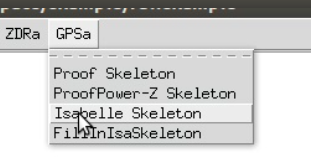
\includegraphics[scale=0.45]{Figures/fullexample/isabelskeleton.png}
\caption{The Isabelle skeleton button the interface which allows the user to generate an Isabelle skeleton of their specification. \label{fig:isabutton}}
\end{figure}

 The Isabelle skeleton consits of the information generated in the general proof skeleton along with the environment to begin an Isabelle theory. It contains comments in between \verb|(* .. *)| paranthesis to show the parts which need to be filled in either by using the \gls{zcga} document or by the user. Figure \ref{fig:isaFullexample} shows the automatically generated Isabelle skeleton for our example.

\begin{figure}[H]
\centering
\begin{minipage}{0.45\textwidth}
\centering
\begin{scriptsize}
\begin{BVerbatim}
theory gpsafullexample
imports 
Main 
begin 
record SS1 = 
(*DECLARATIONS*)
locale fullexample = 
fixes (*GLOBAL DECLARATIONS*) 
begin
definition PRE2 :: 
 "(*PRE2_TYPES*) => bool"
where 
"PRE2 (*PRE2_VARIABLES*) == (*PRECONDITION*) "
definition PRE1 :: 
 "(*PRE1_TYPES*) => bool"
where 
"PRE1 (*PRE1_VARIABLES*) == (*PRECONDITION*) "
\end{BVerbatim}
\end{scriptsize}
\end{minipage}\hfill
\begin{minipage}{0.45\textwidth}
\begin{scriptsize}
\begin{BVerbatim}
definition CS0 :: 
"(*CS0_TYPES*) => bool"
where 
"CS0 (*CS0_VARIABLES*) == True"
definition CS1 :: 
 "(*CS1_TYPES*) => bool"
where 
"CS1 (*CS1_VARIABLES*) == (PO1)"
lemma TS1: 
"(*TS1_EXPRESSION*)"
sorry
end
end
\end{BVerbatim}
\end{scriptsize}
\end{minipage}
\caption{Isabelle proof skeleton. \label{fig:isaFullexample}}
\end{figure}

\subsection{Isabelle Skeleton Filled in}

Using the \gls{zcga} annotated document and the Isabelle skeleton described in the previous section. The user can then automatically fill in the missing information which is needed between the comment parenthesis \verb|(* ...*)|. This is the final step which is automated by the program and the user can click on the \gls{gpsa} button on the main menu bar in the inerface and then click on `\texttt{FillInIsa Skeleton}' in the sub menu (shown in figure \ref{fig:fillinisa}).

\begin{figure}[H]
\centering
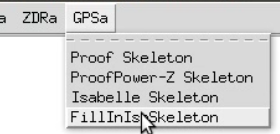
\includegraphics[scale=0.45]{Figures/fullexample/fillinisa.png}
\caption{The Fill in Isabelle Skeleton button the interface which allows the user to fill in the skeleton they previously created. \label{fig:fillinisa}}
\end{figure}

Figure \ref{fig:fillinFullexample} shows our example with a filled in Isabelle skeleton. It is important to note that the program also changes some of the syntax from \LaTeX{} to Isabelle so that it is fully parsable by Isabelle.

\begin{figure}[H]
\centering
\begin{minipage}{0.45\textwidth}
\centering
\begin{scriptsize}
\begin{BVerbatim}
theory gpsafullexample
imports 
Main 
begin 
record VMSTATE = 
STOCK :: nat
TAKINGS :: nat
locale fullexample = 
fixes price :: nat
and stock :: nat
and takings :: nat
begin
definition some_stock :: 
" bool"
where 
"some_stock  = (stock > 0) "
definition exact_cash :: 
 "nat => bool"
where 
"exact_cash cash_tendered = 
(cash_tendered = price) "
definition VM_operation :: 
"VMSTATE => VMSTATE => nat => nat => 
nat => nat => nat => bool"
where 
"VM_operation vmstate vmstate' stock'
takings' cash_tendered 
cash_refunded bars_delivered == True"
\end{BVerbatim}
\end{scriptsize}
\end{minipage}\hfill
\begin{minipage}{0.45\textwidth}
\begin{scriptsize}
\begin{BVerbatim}
definition VM_sale :: 
 "VMSTATE => nat => nat => nat => 
 VMSTATE => nat => nat => bool"
where 
"VM_sale vmstate' stock' bars_delivered
cash_tendered vmstate 
takings' cash_refunded == ((
(stock' = stock - 1) 
\<and> (bars_delivered = 1) 
\<and> (cash_refunded = cash_tendered - price) 
\<and> (takings' = takings + price)))"
lemma VM1: 
"(exact_cash cash_tendered)
\<and> (some_stock )
\<and> (VM_sale vmstate' stock' 
bars_delivered cash_tendered 
vmstate takings' cash_refunded)"
sorry
end
end
\end{BVerbatim}
\end{scriptsize}
\end{minipage}
\caption{Filled In proof skeleton. \label{fig:fillinFullexample}}
\end{figure}

\section{Full Proof}

The next part is to prove any existing lemmas from the filled in Isabelle Skelton or add new lemma's to prove safety properties about the specification. However, this final stage is difficult to automate with \gls{zmath} as everyone has different properties they wish to prove and all specification are different themselves. So the final step will need some theorem prover knowledge, but not as much as translating the specification and proving it in one step as the specification is already put into the theorem prover syntax. In this case the user may wish to use theorem prover tools which already exist such as Sledgehammer \cite{sledgehammer} to help them prove the properties. An example is shown in figure \ref{fig:propertyproof} of a property and it's proof in Isabelle of the vending machine example.

\begin{figure}[H]
\centering
\begin{scriptsize}
\begin{BVerbatim}
lemma VM3_ok:
"(\<exists> stock' takings cash_refunded bars_delivered.
(VM3 cash_tendered stock takings stock' takings' cash_refunded
bars_delivered)
\<longrightarrow>
((takings' - takings) \<ge> price * (stock - stock' )))"
apply (unfold VM3_def VM1_def VM2_def exact_cash_def some_stock_def
  VM_sale_def VM_nosale_def insufficient_cash_def)
apply auto
done
\end{BVerbatim}
\end{scriptsize}
\caption{An example of a property and it's proof for the Vending Machine example. \label{fig:propertyproof}}
\end{figure}

\section{Conclusion}
In this chapter we have taken a single specification and shown the entire path from the raw specification to it's translation in Isabelle. We have shown the \LaTeX{} code and the compiled output for the raw specification, \gls{zcga} annotated specification and \gls{zdra} annotated specification. We have shown screenshots of the interface to demonstrate of how to check for each step of correctness. The dependency and goto graphs where automatically demonstrated and displayed. Then the general proof skeleton, (which shows the order the instances must be in to input into a theorem prover) was displayed. We then generated an Isabelle proof skeleton for the vending machine and automatically filled it in using the \gls{zmath} program. In the final section we explained that it would be difficult to automate a proof due to the fact that the lemma's which need to be proved for a specification will vary due to the nature of the specification and the user who wishes to prove them. 

In the next chapter we analyse the differences between translating a specification in one step and translating a specification using the \gls{zmath} method.